%%%%%%%%%%%%%%%%%%%%%%%%%%%%%%%%%%%%%%%%%
% Beamer Presentation
% LaTeX Template
% Version 2.0 (March 8, 2022)
%
% This template originates from:
% https://www.LaTeXTemplates.com
%
% Author:
% Vel (vel@latextemplates.com)
%
% License:
% CC BY-NC-SA 4.0 (https://creativecommons.org/licenses/by-nc-sa/4.0/)
%
%%%%%%%%%%%%%%%%%%%%%%%%%%%%%%%%%%%%%%%%%

%----------------------------------------------------------------------------------------
%	PACKAGES AND OTHER DOCUMENT CONFIGURATIONS
%----------------------------------------------------------------------------------------

\documentclass[
	11pt, % Set the default font size, options include: 8pt, 9pt, 10pt, 11pt, 12pt, 14pt, 17pt, 20pt
	%t, % Uncomment to vertically align all slide content to the top of the slide, rather than the default centered
	%aspectratio=169, % Uncomment to set the aspect ratio to a 16:9 ratio which matches the aspect ratio of 1080p and 4K screens and projectors
]{beamer}

\graphicspath{{Images/}{./}} % Specifies where to look for included images (trailing slash required)

\usepackage{booktabs} % Allows the use of \toprule, \midrule and \bottomrule for better rules in tables

%----------------------------------------------------------------------------------------
%	SELECT LAYOUT THEME
%----------------------------------------------------------------------------------------

% Beamer comes with a number of default layout themes which change the colors and layouts of slides. Below is a list of all themes available, uncomment each in turn to see what they look like.

%\usetheme{default}
%\usetheme{AnnArbor}
%\usetheme{Antibes}
%\usetheme{Bergen}
%\usetheme{Berkeley}
%\usetheme{Berlin}
%\usetheme{Boadilla}
%\usetheme{CambridgeUS}
%\usetheme{Copenhagen}
%\usetheme{Darmstadt}
%\usetheme{Dresden}
%\usetheme{Frankfurt}
%\usetheme{Goettingen}
%\usetheme{Hannover}
%\usetheme{Ilmenau}
%\usetheme{JuanLesPins}
%\usetheme{Luebeck}
\usetheme{Madrid}
%\usetheme{Malmoe}
%\usetheme{Marburg}
%\usetheme{Montpellier}
%\usetheme{PaloAlto}
%\usetheme{Pittsburgh}
%\usetheme{Rochester}
%\usetheme{Singapore}
%\usetheme{Szeged}
%\usetheme{Warsaw}

%----------------------------------------------------------------------------------------
%	SELECT COLOR THEME
%----------------------------------------------------------------------------------------

% Beamer comes with a number of color themes that can be applied to any layout theme to change its colors. Uncomment each of these in turn to see how they change the colors of your selected layout theme.

%\usecolortheme{albatross}
%\usecolortheme{beaver}
%\usecolortheme{beetle}
%\usecolortheme{crane}
%\usecolortheme{dolphin}
%\usecolortheme{dove}
%\usecolortheme{fly}
%\usecolortheme{lily}
%\usecolortheme{monarca}
%\usecolortheme{seagull}
%\usecolortheme{seahorse}
%\usecolortheme{spruce}
%\usecolortheme{whale}
%\usecolortheme{wolverine}

%----------------------------------------------------------------------------------------
%	SELECT FONT THEME & FONTS
%----------------------------------------------------------------------------------------

% Beamer comes with several font themes to easily change the fonts used in various parts of the presentation. Review the comments beside each one to decide if you would like to use it. Note that additional options can be specified for several of these font themes, consult the beamer documentation for more information.

\usefonttheme{default} % Typeset using the default sans serif font
%\usefonttheme{serif} % Typeset using the default serif font (make sure a sans font isn't being set as the default font if you use this option!)
%\usefonttheme{structurebold} % Typeset important structure text (titles, headlines, footlines, sidebar, etc) in bold
%\usefonttheme{structureitalicserif} % Typeset important structure text (titles, headlines, footlines, sidebar, etc) in italic serif
%\usefonttheme{structuresmallcapsserif} % Typeset important structure text (titles, headlines, footlines, sidebar, etc) in small caps serif

%------------------------------------------------

%\usepackage{mathptmx} % Use the Times font for serif text
\usepackage{palatino} % Use the Palatino font for serif text

%\usepackage{helvet} % Use the Helvetica font for sans serif text
\usepackage[default]{opensans} % Use the Open Sans font for sans serif text
%\usepackage[default]{FiraSans} % Use the Fira Sans font for sans serif text
%\usepackage[default]{lato} % Use the Lato font for sans serif text
\usepackage[yyyymmdd]{datetime}
\usepackage[french]{babel}

%----------------------------------------------------------------------------------------
%	SELECT INNER THEME
%----------------------------------------------------------------------------------------

% Inner themes change the styling of internal slide elements, for example: bullet points, blocks, bibliography entries, title pages, theorems, etc. Uncomment each theme in turn to see what changes it makes to your presentation.

%\useinnertheme{default}
\useinnertheme{circles}
%\useinnertheme{rectangles}
%\useinnertheme{rounded}
%\useinnertheme{inmargin}

%----------------------------------------------------------------------------------------
%	SELECT OUTER THEME
%----------------------------------------------------------------------------------------

% Outer themes change the overall layout of slides, such as: header and footer lines, sidebars and slide titles. Uncomment each theme in turn to see what changes it makes to your presentation.

%\useoutertheme{default}
%\useoutertheme{infolines}
%\useoutertheme{miniframes}
%\useoutertheme{smoothbars}
%\useoutertheme{sidebar}
%\useoutertheme{split}
%\useoutertheme{shadow}
%\useoutertheme{tree}
%\useoutertheme{smoothtree}

%\setbeamertemplate{footline} % Uncomment this line to remove the footer line in all slides
%\setbeamertemplate{footline}[page number] % Uncomment this line to replace the footer line in all slides with a simple slide count

%\setbeamertemplate{navigation symbols}{} % Uncomment this line to remove the navigation symbols from the bottom of all slides

%----------------------------------------------------------------------------------------
%	PRESENTATION INFORMATION
%----------------------------------------------------------------------------------------

\title[Initation Recherche]{Création de diffférentes IA en utilisant une architecture I2A} % The short title in the optional parameter appears at the bottom of every slide, the full title in the main parameter is only on the title page

\subtitle{Dans le contexte du jeu Sokoban} % Presentation subtitle, remove this command if a subtitle isn't required

\author[Thomas Guyomard / Jérémy Tremblay]{Thomas Guyomard - Jérémy Tremblay} % Presenter name(s), the optional parameter can contain a shortened version to appear on the bottom of every slide, while the main parameter will appear on the title slide

\institute[]{Université du Littoral Côte d'Opale\\ \smallskip \textit{Encadrant : M. Jérôme Buisine}} % Your institution, the optional parameter can be used for the institution shorthand and will appear on the bottom of every slide after author names, while the required parameter is used on the title slide and can include your email address or additional information on separate lines

\date[\today]{\today} % Presentation date or conference/meeting name, the optional parameter can contain a shortened version to appear on the bottom of every slide, while the required parameter value is output to the title slide

%----------------------------------------------------------------------------------------

\begin{document}

%----------------------------------------------------------------------------------------
%	TITLE SLIDE
%----------------------------------------------------------------------------------------

\begin{frame}
	\titlepage % Output the title slide, automatically created using the text entered in the PRESENTATION INFORMATION block above
\end{frame}

%----------------------------------------------------------------------------------------
%	TABLE OF CONTENTS SLIDE
%----------------------------------------------------------------------------------------

% The table of contents outputs the sections and subsections that appear in your presentation, specified with the standard \section and \subsection commands. You may either display all sections and subsections on one slide with \tableofcontents, or display each section at a time on subsequent slides with \tableofcontents[pausesections]. The latter is useful if you want to step through each section and mention what you will discuss.

\begin{frame}
	\frametitle{Sommaire} % Slide title, remove this command for no title
	
	\tableofcontents % Output the table of contents (all sections on one slide)
	%\tableofcontents[pausesections] % Output the table of contents (break sections up across separate slides)
\end{frame}

%----------------------------------------------------------------------------------------
%	PRESENTATION BODY SLIDES
%----------------------------------------------------------------------------------------

 % Sections are added in order to organize your presentation into discrete blocks, all sections and subsections are automatically output to the table of contents as an overview of the talk but NOT output in the presentation as separate slides

%------------------------------------------------

\section{Références}

\begin{frame}
	\frametitle{Références}
	
	Sébastien Racanière, Théophane Weber, David P. Reichert, Lars Buesing, Arthur Guez, Danilo Rezende, Adria Puigdomènech Badia, Oriol Vinyals, Nicolas Heess, Yujia Li, Razvan Pascanu, Peter Battaglia, Demis Hassabis, David Silver, Daan Wierstra, "Imagination-Augmented Agents for Deep Reinforcement Learning", DeepMind, arXiv:1707.06203v2 [cs.LG] 14 Feb 2018
	
\end{frame}

%------------------------------------------------
\section{Présentation du jeu Sokoban}

\begin{frame}
	\frametitle{Présentation du jeu Sokoban}
	
	Jeu de \alert{réflexion}. le joueur doit ranger des caisses sur des cases cibles.
	\bigskip % Vertical whitespace
	
	\begin{itemize}
		\item Le personnage peut réaliser neuf opérations :
        \begin{itemize}
            \item 4 opérations concernent le déplacement dans une case adjacente à lui (droite, gauche, haut, bas).
            \item 4 opérations concernent l'action de pousser une caisse sur une case adjacente à lui dans la direction de son mouvement (droite, haut, gauche, bas), sauf si celle-ci est bloquée par un obstacle quelconque.
            \item La dernière action vide : ne rien faire.
		\end{itemize}
	\end{itemize}

	\bigskip % Vertical whitespace
	
	Une fois toutes les caisses rangées le niveau est validé et ainsi de suite jusqu'à la fin de tout les niveaux.
	
\end{frame}

%------------------------------------------------
\section{Environnement d'étude}

\begin{frame}
	\frametitle{Environnement d'étude}
	
	\begin{columns}[c] % The "c" option specifies centered vertical alignment while the "t" option is used for top vertical alignment
		\begin{column}{0.45\textwidth} % Left column width
			\textbf{Environnement de travail}
			\begin{enumerate}
				\item Python
				\item Gym
				\item Plusieurs modes de jeu
			\end{enumerate}
		\end{column}
		\begin{column}{0.5\textwidth} % Right column width
	
		\begin{figure}
			\centering
			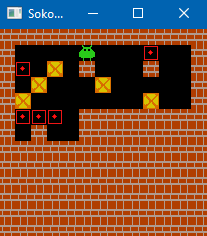
\includegraphics[width=0.9\linewidth]{Images/sokoban.png}
			\caption{Capture d'écran du jeu Sokoban}
		\end{figure}
		\end{column}
	\end{columns}
\end{frame}
%------------------------------------------------
\section{Agents Augmentés par l'Imagination}

\begin{frame}
	\frametitle{Agents Augmentés par l'Imagination \ / (I2A)}
	
	\smallskip % Vertical whitespace

	\begin{definition}
	\alert{L'apprentissage par renforcement avec augmentation par l'imagination} appelée \alert{I2A} est une approche du domaine de l'intelligence artificielle permettant d'améliorer la prise de décision des agents d'apprentissage.
	Les agents combinent l'apprentissage automatique avec et sans modèles avec des générations de scénarios pour anticiper des situations inédites et proposer des solutions optimales.
	\end{definition}
	
	\smallskip % Vertical whitespace

\end{frame}

%------------------------------------------------
\section{Fonctionnement des Agents Augmentés par Imagination}

\begin{frame}
	\frametitle{Fonctionnement des Agents Augmentés par Imagination}
	
	\smallskip % Vertical whitespace

	\begin{figure}
		\centering
		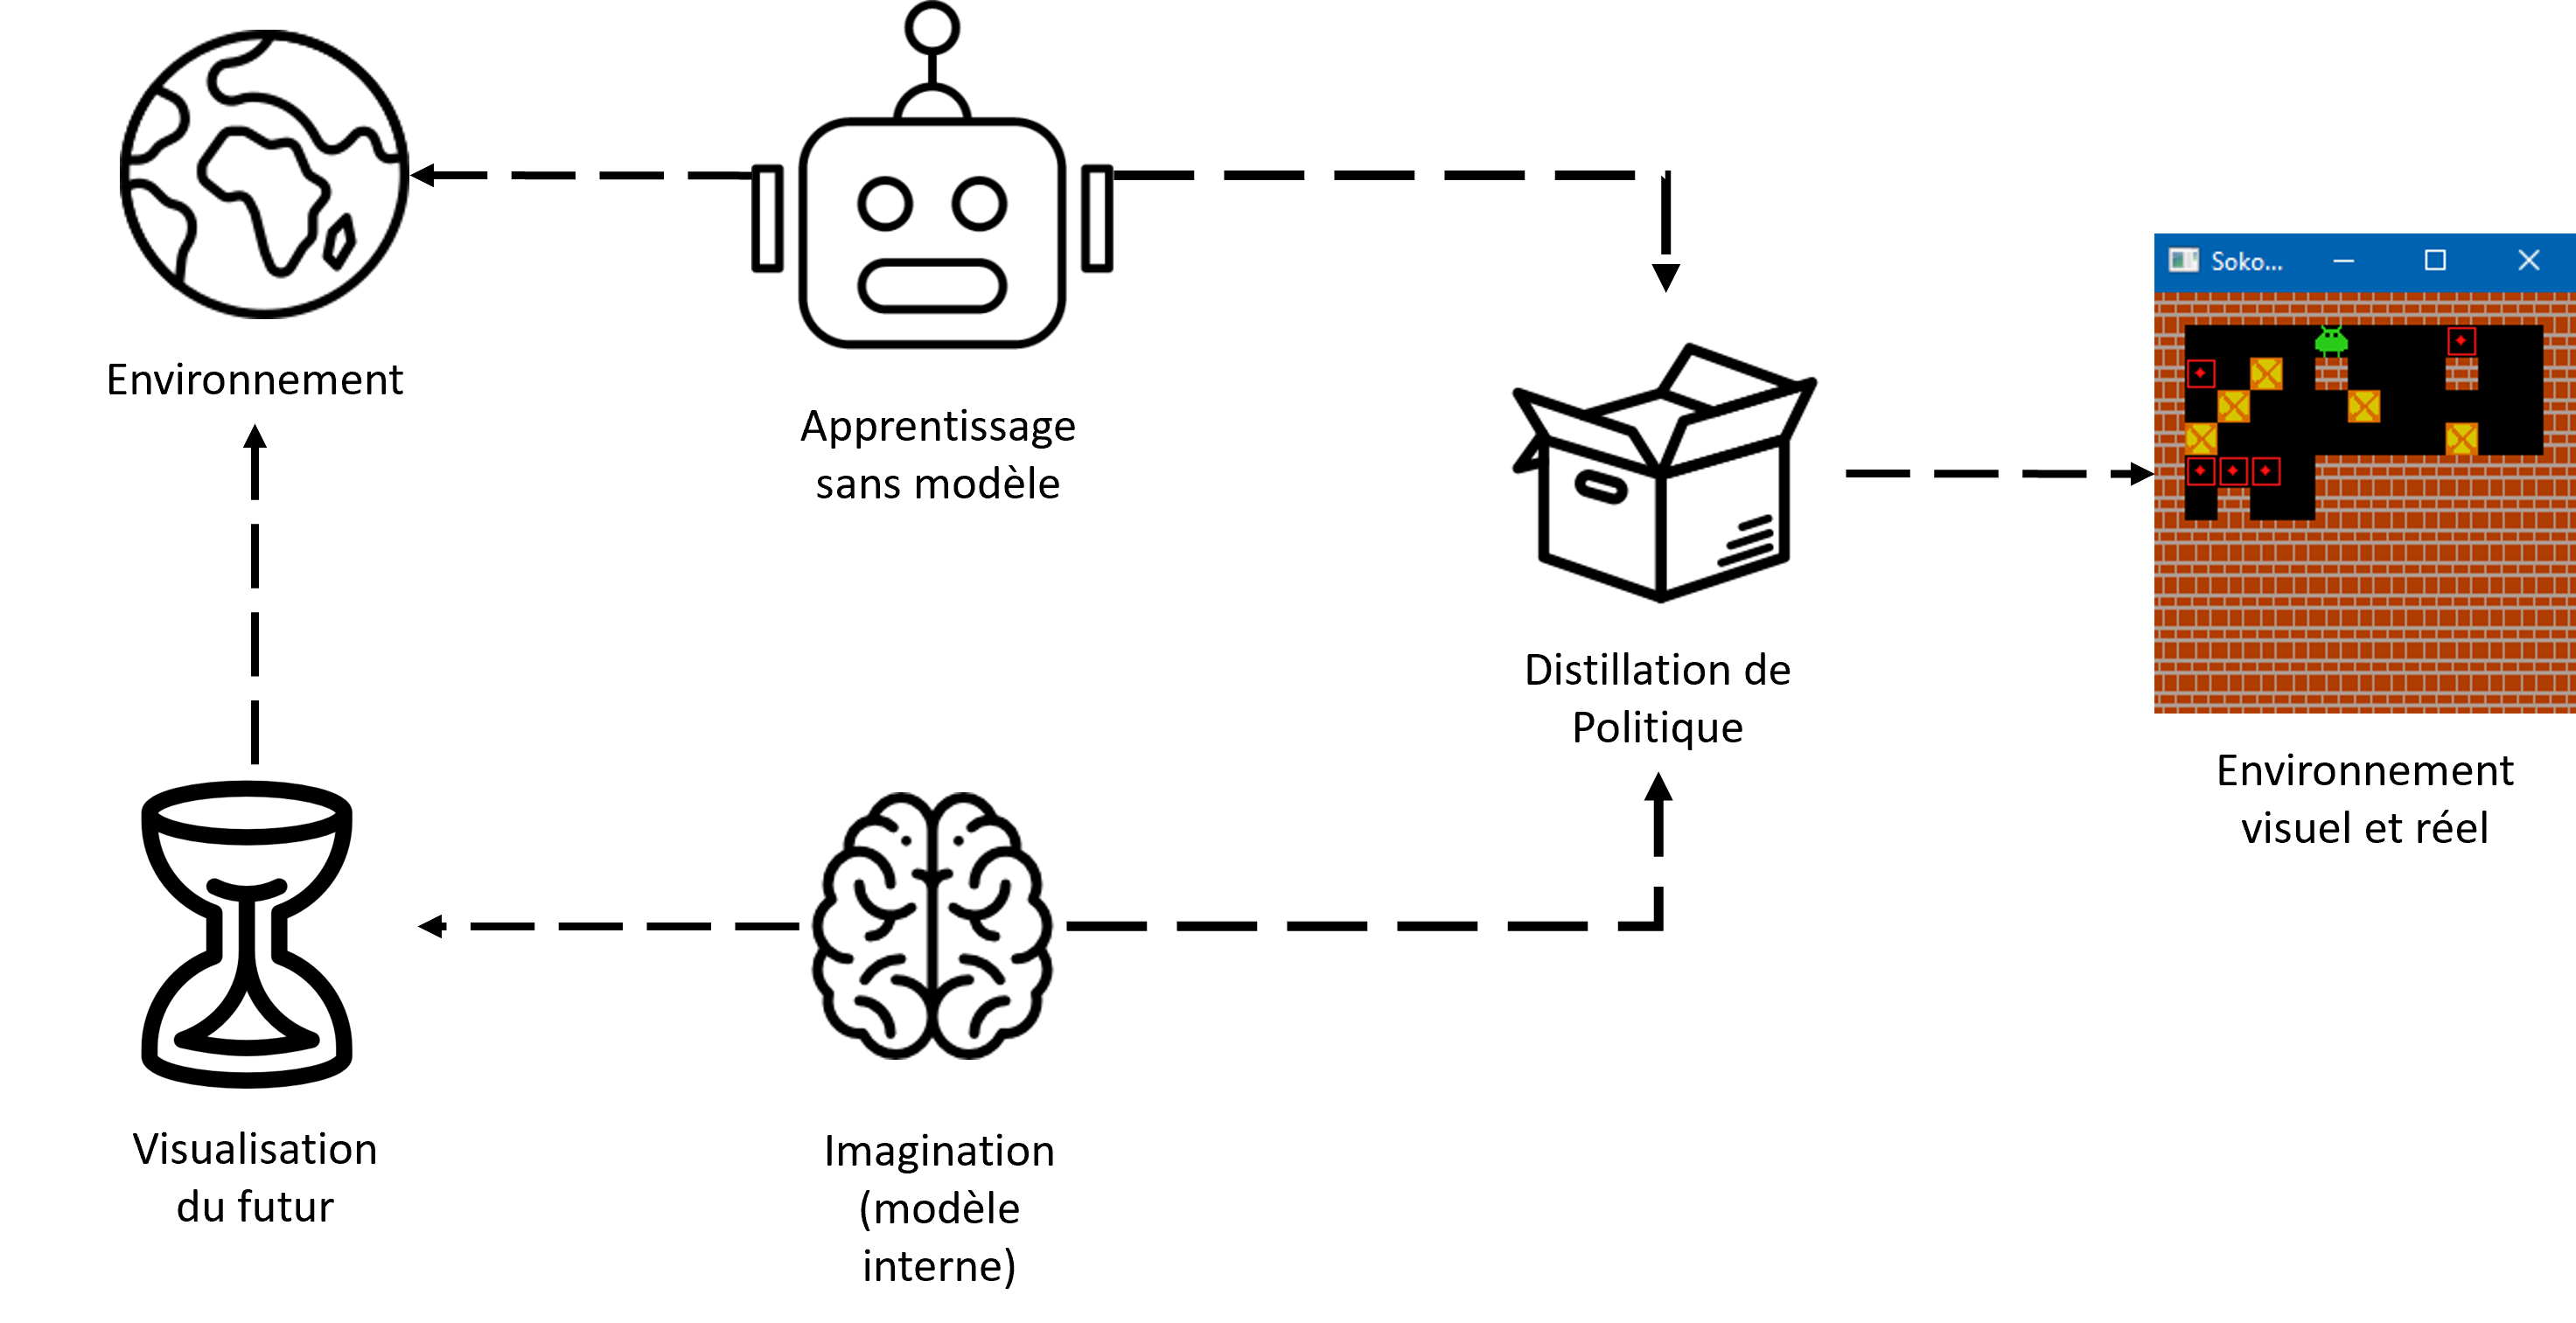
\includegraphics[width=1.0\linewidth]{Images/schema_i2a.png}
		\caption{Schéma récapitulatif de l'approche I2A.}
	\end{figure}
	
	\smallskip % Vertical whitespace

\end{frame}

%------------------------------------------------
\section{Performances de différents modèles}

\begin{frame}
	\frametitle{Performances de différents modèles}
	
	\smallskip % Vertical whitespace

	\begin{block}{Informations}
		Les différents modèles ne performent pas de la même manière au jeu du Sokoban.
	\end{block}

	\begin{figure}
		\centering
		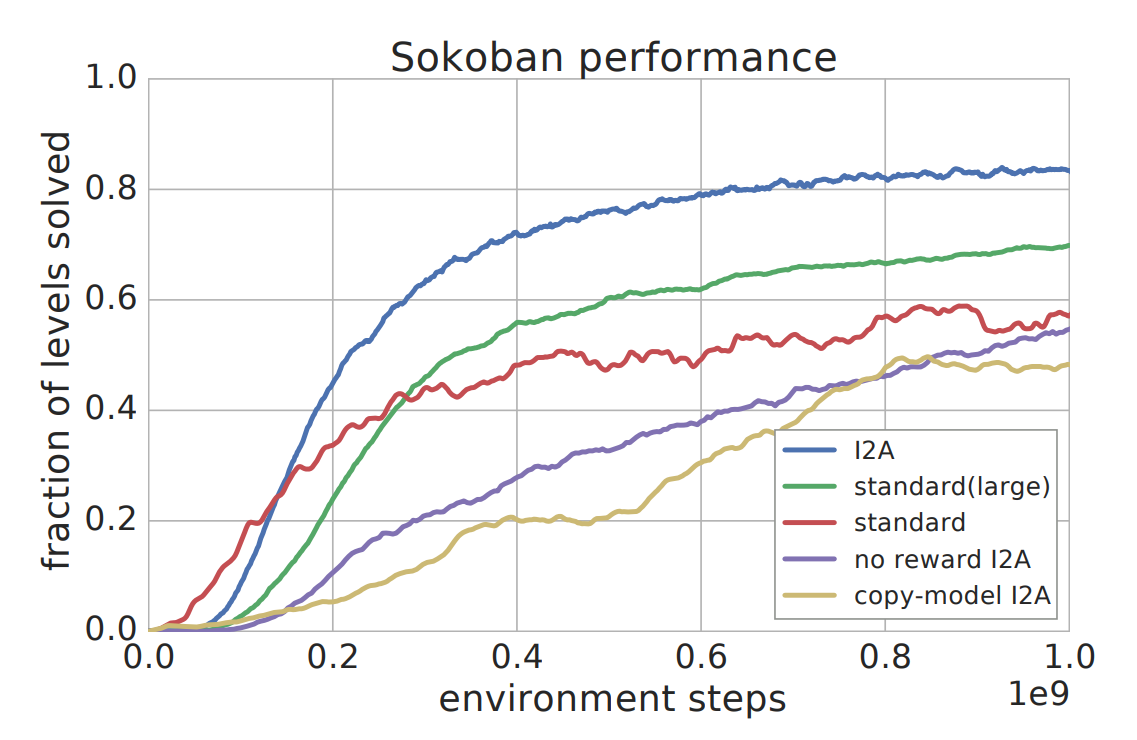
\includegraphics[width=0.65\linewidth]{Images/sokoban_performance.png}
		\caption{Schéma représentant les succès de différents modèles au jeu du sokoban.}
	\end{figure}
	
	\smallskip % Vertical whitespace

\end{frame}

%------------------------------------------------
\section{Comparaison d'efficacité de l'imagination}

\begin{frame}{Comparaison d'efficacité de l'imagination}
    \begin{columns}
        \begin{column}{\textwidth}
            \begin{table}
                \centering
                \begin{tabular}{l|ccccccc}
                    Boxes & 1 & 2 & 3 & 4 & 5 & 6 & 7 \\
                    \hline
                    I2A (\%) & 99.5 & 97 & 92 & 87 & 77 & 66 & 53 \\
                    Standard (\%) & 97 & 87 & 72 & 60 & 47 & 32 & 23 \\
					\caption{Généralisation de I2A à des environnements avec différents nombres de boîtes.}
                \end{tabular}
				
            \end{table}

            \begin{table}
                \centering
                \begin{tabular}{l|ccccccc}
                    I2A@87 & $\sim$ 1400 \\
                    I2A MC search @95 & $\sim$ 4000 \\
                    MCTS@87 & $\sim$ 25000 \\
                    MCTS@95 & $\sim$ 100000 \\
                    Random search & $\sim$ millions \\
                \end{tabular}
				\caption{Efficacité de l'imagination pour différentes architectures.}
            \end{table}
        \end{column}
    \end{columns}
\end{frame}

%------------------------------------------------

\section{Q-learning avec une représentation en tableau}

\begin{frame}
	\frametitle{Q-learning avec une représentation en tableau}
	
	\begin{block}{Definitions}
		Le Q-learning facilite les décisions séquentielles. Grâce à un tableau, chaque cellule stocke la valeur Q, qui est mise à jour lorsqu'un agent prend une action dans un état donné qui aide ainsi à l'amélioration petit à petit de la politique de prise de décision.
	\end{block}
	
	\smallskip % Vertical whitespace

	\begin{figure}
		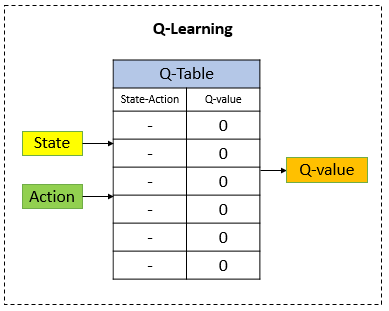
\includegraphics[width=0.4\linewidth]{Images/q_learning.png}
		\caption{Schéma du fonctionnement du Q-Learning.}
	\end{figure}

	
\end{frame}
%------------------------------------------------

\section{Deep Q-Learning avec un réseau de neurones}

\begin{frame}
	\frametitle{Deep Q-Learning avec un réseau de neurones}
	
	\begin{block}{Definitions}
		Le \alert{Deep Q-Learning} est une extension de Q-Learning qui utilise des réseaux de neurones profonds pour gérer des d'états et d'actions plus importants que le Q-Learning classique.
	\end{block}

	\smallskip % Vertical whitespace

	\begin{figure}
		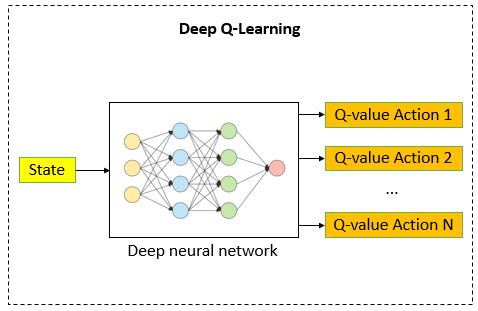
\includegraphics[width=0.5\linewidth]{Images/deep_q_learning.png}
		\caption{Schéma du fonctionnement du Deep Q-Learning.}
	\end{figure}
	
\end{frame}

%------------------------------------------------
\section{Parallèle entre Sokoban et les I2A}

\begin{frame}
	\frametitle{Parallèle entre Sokoban et les I2A}

	\begin{block}{Objectifs}
		Objectif : entraîner un agent étant en capacité de jouer et d'évoluer dans le jeu du Sokoban.
		Problématique : Comment l'I2A peut-elle être appliquée pour guider les actions dans un environnement complexe ?
	\end{block}

	\smallskip % Vertical whitespace
	
	\begin{itemize}
		\item 9 actions mais une infinités de cartes de tailles différentes et parfois plusieurs solutions possibles.
		\item Il faut adapter les concepts de l'I2A au jeu du Sokoban afin d'obtenir un modèle performant.
		\item Plan d'action : 
		\begin{itemize}
			\item Distillation de la politique pour combiner apprentissage sans modèle et avec modèle.
			\item Utilisation de l'imagination pour guider les actions dans l'environnement.
			\item Ajout de visuels de l'environnement du jeu avec traitement d'image afin d'améliorer les résultats.
		\end{itemize}
	\end{itemize}
	
\end{frame}

%------------------------------------------------
\section{Plan de Travail}

\begin{frame}{Plan de Travail}
    \begin{table}
        \centering
		\small
        \begin{tabular}{|c|p{8cm}|}
            \hline
            1 & Compréhension et test de l'environnement Gym Sokoban. \\
            \hline
            2 & Recherche et compréhension des différentes approches (Q-learning, MCTS, Deep Q-Learning). \\
            \hline
            3 & Développement de différents modèles d'apprentissage automatique (Q-learning, Deep Q-learning...). \\
            \hline
            4 & Utilisation de l'approche I2A dans notre jeu. \\
            \hline
            5 & Comparaison des performances avec des modèles comme MCTS pour évaluer l'efficacité relative. \\
            \hline
            6 & Si possible, explorer la possibilité d'utiliser les représentations visuelles de Gym Sokoban pour enrichir la planification. \\
            \hline
            7 & Tester l'agent sur différents niveaux afin d'évaluer sa capacité de généralisation. \\
            \hline
            8 & Analyser les performances de chaque approche, en mettant en évidence les forces et les faiblesses dans le contexte de Sokoban. \\
            \hline
        \end{tabular}
    \end{table}
\end{frame}

%----------------------------------------------------------------------------------------
%	CLOSING SLIDE
%----------------------------------------------------------------------------------------

\begin{frame}[plain] % The optional argument 'plain' hides the headline and footline
	\begin{center}
		{\Huge Merci pour votre attention.}
		
	\end{center}
\end{frame}
%------------------------------------------------
\section{AUTRE}

%----------------------------------------------------------------------------------------

\end{document} 